\clearpage
\chapter{Results}

\section{Correlation of Parameters} \label{section:corrofparams}

We observe correlation between two parameters using the statistical definition of the correlation coefficient ($\rho_{X,Y}$), defined in Eqn. \ref{eqn:correlation}.

\begin{equation}
\rho_{X,Y} = \dfrac{cov(X,Y)}{\sigma_X\sigma_Y}
\label{eqn:correlation}
\end{equation}

\textit{cov} represents covariance, and \hl{$\sigma_{S}$} represents the standard deviation of a set \hl{$S$}. The correlation coefficient is unitless, and measured from -1.0 $<$ $\rho_{X,Y}$ $<$ 1.0. A correlation coefficient of 0 indicates the variables X and Y are uncorrelated, while -1.0 indicates the variables are perfectly inversely correlated; likewise, a correlation coefficient of 1.0 means X and Y are perfectly correlated. Correlation coefficient is used to estimate an environmental parameter's potential usefulness for calculating a new \textit{coneR1} for use in an arbitrary environment. We represent the correlation between \textit{coneR1}* and $\alpha$ as $\rho_{\alpha}$.

\subsection{\textit{coneR1}* and Average Attenuation} \label{section:coner1andatten}

Both attenuation models ($\alpha_{dB}$ and $\alpha_{\%\Delta}$) were considered for correlation against the \textit{coneR1}* values of a dataset. Correlation $\rho_{\alpha}$ is represented for both attenuation models as $\rho_{dB}$ and $\rho_{\%\Delta}$ respectively. Results for both are illustrated in Figure \ref{fig:corr_db} and Figure \ref{fig:corr_rgb}. Tables \ref{table:corr_db} and \ref{table:corr_rgb} present correlation coefficients for each dataset for $\alpha_{dB}$ and $\alpha_{\%\Delta}$.

% dB correlation
\begin{figure}
  \centering
  \begin{subfigure}{1\linewidth}
  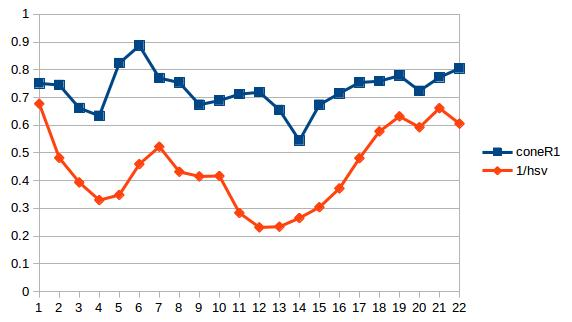
\includegraphics[width=1\linewidth]{figures/correlations/db/room_hsv.jpg}
  \caption{aton\_room}
\end{subfigure}
\hfill
\begin{subfigure}{.49\linewidth}
  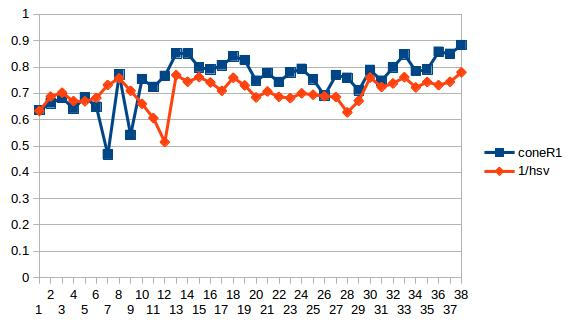
\includegraphics[width=1\linewidth]{figures/correlations/db/campus_hsv.jpg}
  \caption{aton\_campus}
\end{subfigure}
\begin{subfigure}{.49\linewidth}
  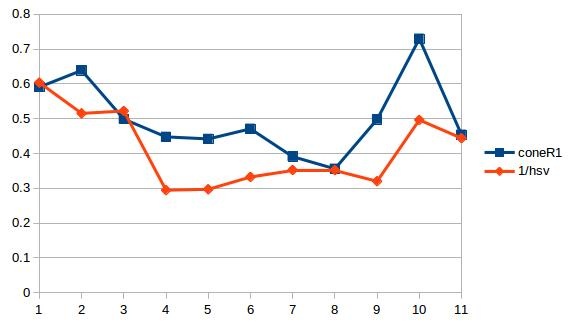
\includegraphics[width=1\linewidth]{figures/correlations/db/pets2_hsv.jpg}
  \caption{PETS2}
\end{subfigure}

\caption{Correlation of $\alpha_{dB}$ (orange) and \textit{coneR1}* (blue) is observed \hl{across all datasets. Three are shown here}. (All results can be found in the appendix)}
\label{fig:corr_db}
\end{figure}

% RGB model
\begin{figure}
  \centering
  \begin{subfigure}{1\linewidth}
  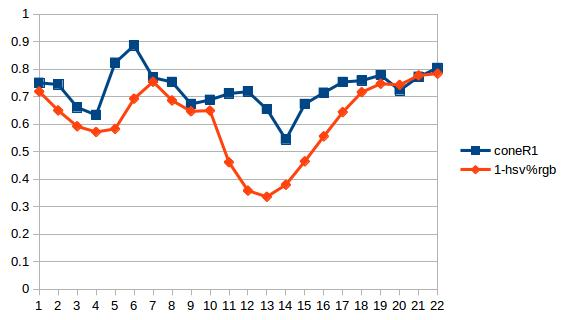
\includegraphics[width=1\linewidth]{figures/correlations/rgb/room_hsv.jpg}
  \caption{aton\_room}
\end{subfigure}
\hfill
\begin{subfigure}{.49\linewidth}
  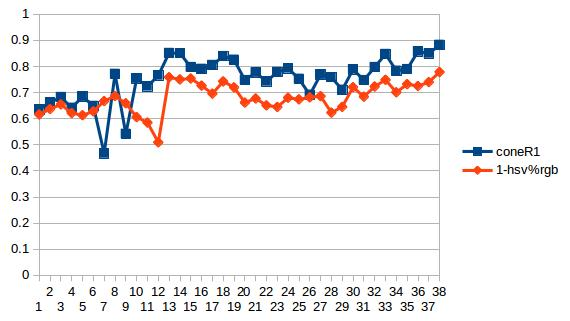
\includegraphics[width=1\linewidth]{figures/correlations/rgb/campus_hsv.jpg}
  \caption{aton\_campus}
\end{subfigure}
\begin{subfigure}{.49\linewidth}
  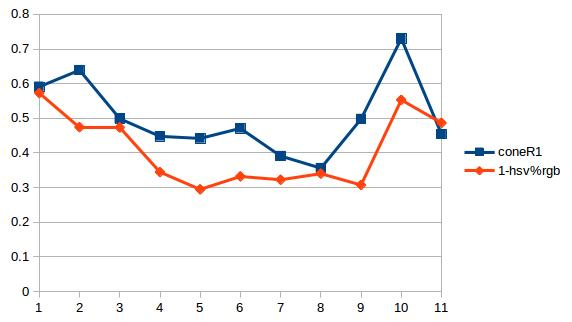
\includegraphics[width=1\linewidth]{figures/correlations/rgb/pets2_hsv.jpg}
  \caption{PETS2}
\end{subfigure}

\caption{\hl{Likewise,} correlation of $\alpha_{\%\Delta}$ (orange) and \textit{coneR1}* (blue) is observed \hl{across all datasets with three shown here.} (All results can be found in the appendix)}
\label{fig:corr_rgb}
\end{figure}

% Table Form (dB)
\begin{table}
\centering
\begin{tabular}{ |c|c|c|c| }
	\hline
	%\textbf{Dataset} & \textbf{$\sigma_{coneR1}$} & \textbf{$\sigma_{dB}$} & \textbf{$\rho$} \\
	\textbf{Dataset} & \textbf{$\rho_{\alpha}$} \\
	\hline
	\hline
	%\textbf{PETS1} & 0.19855 \\
	\textbf{PETS1} & 0.199 \\
	\hline
	%\textbf{PETS2} & 0.67058 \\
	\textbf{PETS2} & 0.671 \\
	\hline
	%\textbf{aton\_highway1} & 0.68368 \\
	\textbf{aton\_highway1} & 0.684 \\
	\hline
	%\textbf{aton\_highway3} & 0.74241 \\
	\textbf{aton\_highway3} & 0.742 \\
	\hline
	%\textbf{aton\_room} & 0.54775 \\
	\textbf{aton\_room} & 0.548 \\
	\hline
	%\textbf{aton\_campus} & 0.35996 \\
	\textbf{aton\_campus} & 0.360 \\
	\hline
	%\textbf{aton\_hallway} & 0.65615 \\
	\textbf{aton\_hallway} & 0.656 \\
	\hline
	%\textbf{aton\_lab} &  0.69540 \\
	\textbf{aton\_lab} &  0.695 \\
	\hline
\end{tabular}
\caption{Datasets and their $\alpha_{dB}$ correlations to \textit{coneR1}*.}
\label{table:corr_db}
\end{table}

% Table Form (RGB)
\begin{table}
\centering
\begin{tabular}{ |c|c|c|c| }
	\hline
	\textbf{Dataset} & \textbf{$\rho_{\%\Delta}$} \\
	\hline
	\hline
	\textbf{PETS1} & 0.184 \\
	\hline
	\textbf{PETS2} & 0.743 \\
	\hline
	\textbf{aton\_highway1} & 0.592 \\
	\hline
	\textbf{aton\_highway3} & 0.801 \\
	\hline
	\textbf{aton\_room} & 0.623 \\
	\hline
	\textbf{aton\_campus} & 0.564 \\
	\hline
	\textbf{aton\_hallway} & 0.690 \\
	\hline
	\textbf{aton\_lab} & 0.551 \\
	\hline
\end{tabular}
\caption{Datasets and their $\alpha_{\%\Delta}$ correlations to \textit{coneR1}*.}
\label{table:corr_rgb}
\end{table}

Both Tables \ref{table:corr_db} and \ref{table:corr_rgb} demonstrate significant correlation between \textit{coneR1}* and $\alpha$, consistent across all datasets. \hl{To provide contrast}, an arbitrary variable (number of normal SIFT features detected) has been correlated against \textit{coneR1}* (Table \ref{table:bad_corr}). \hl{In Table \ref{table:bad_corr},} we observe positive and negative correlations, as well as strong and weak correlations.  \hl{Significant correlations are observed, but are inconsistent.} \hl{These tables show} consistent positive $\alpha$ correlations across datasets. Strong and consistent correlation between the two sets implies that both $\alpha_{dB}$ and $\alpha_{\%\Delta}$ will provide a \textit{coneR1}$'$ that will improve shadow removal across the selected datasets.

% Table Form (bad 0.03 correlations)
\begin{table}
\centering
\begin{tabular}{ |c|c|c|c| }
	\hline
	\textbf{Dataset} & \textbf{$\rho_{SIFT}$} \\
	\hline
	\hline
	\textbf{PETS1} & -0.057 \\
	\hline
	\textbf{PETS2} & -0.727 \\
	\hline
	\textbf{aton\_highway1} & 0.009 \\
	\hline
	\textbf{aton\_highway3} & 0.350 \\
	\hline
	\textbf{aton\_room} & -0.079 \\
	\hline
	\textbf{aton\_campus} & 0.218 \\
	\hline
	\textbf{aton\_hallway} & -0.201 \\
	\hline
	\textbf{aton\_lab} & 0.046 \\
	\hline
\end{tabular}
\caption{Datasets and their $SIFT$ correlations to \textit{coneR1}*.}
\label{table:bad_corr}
\end{table}

PETS1 is the primary outlier with a correlation coefficient of approximately 19\% for both attenuation models. While both PETS2 and PETS1 experience illumination change within the extracted samples, PETS2 and \textit{coneR1}* have a correlation coefficient of approximately 74\%. During the illumination change in PETS2, in which the average brightness of the entire scene decreases by 23\%, observed attenuation proportionally decreases by 28\%. We observe \textit{coneR1}* decreases by 37\%. PETS1 experiences a similar illumination change (21\%), and an attenuation change of 32\%, but no significant corresponding fluctuation in \textit{coneR1}*. Illumination and parametric fluctuation was obtained by measuring these values at the beginning and end of the illumination change within the dataset, a range of 22 frames for PETS2, and 45 frames for PETS1. One possible explanation for this discrepancy is that because every pixel is darkened by roughly the same amount due to the illumination shift, the attenuation changes, while the normalized value \textit{coneR1}* does not. However, since this behavior is not evident in PETS2 as well, there are likely undiscovered factors influencing PETS1's poor correlation coefficient.

%PETS1 serves as the primary outlier with a correlation coefficient of approximately 19\% for both attenuation models. One of the primary culprits is the lack of a properly adaptive background model for the dataset, i.e., a frame may contain extreme cloud cover, while its corresponding background model retains its sunny disposition. The resultant of the non-ideal background model is that every pixel contained in the foreground has a greater attenuation when compared to its background pixel, excluding natural cast shadows, whose attenuation remains relatively consistent. This large swing in overall attenuation impacts the amount of pixels considered for candidacy by Physical removal's weak detector. The discrepancy found in the correlation coefficient of PETS1 is the result of the flood of non-shadow candidate pixels. While both PETS2 and PETS1 experience illumination change within the extracted samples, PETS2 does not endure the same measure of disrelation. The illumination change in PETS2 causes less intensity differential, allowing for shadow pixels to remain distinct. 

%\hl{Both $\alpha_{dB}$ and $\alpha_{\%\Delta}$ are illustrated in Figure \ref{fig:corr_compare}} to contrast the trends of \hl{each attenuation model}.
\hl{Figure \ref{fig:corr_compare}}

% Compare RGB to dB
%\begin{figure}
%\centering
%\begin{subfigure}{.49\linewidth}
%  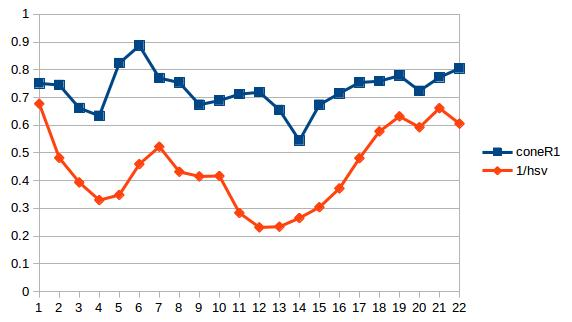
\includegraphics[width=1\linewidth]{figures/correlations/db/room_hsv.jpg}
%  \caption{aton\_room ($\alpha_{dB}$)}
%\end{subfigure}
%\hfill
%\begin{subfigure}{.49\linewidth}
%  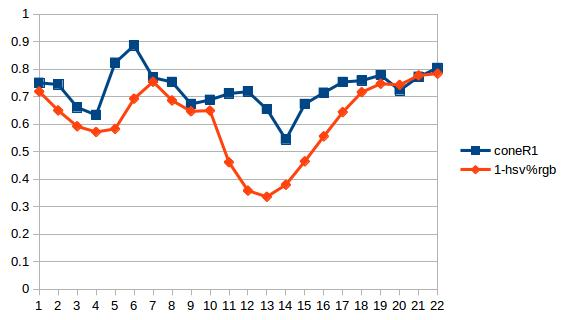
\includegraphics[width=1\linewidth]{figures/correlations/rgb/room_hsv.jpg}
%  \caption{aton\_room ($\alpha_{\%\Delta}$)}
%\end{subfigure}
%\hfill
%\begin{subfigure}{.49\linewidth}
%  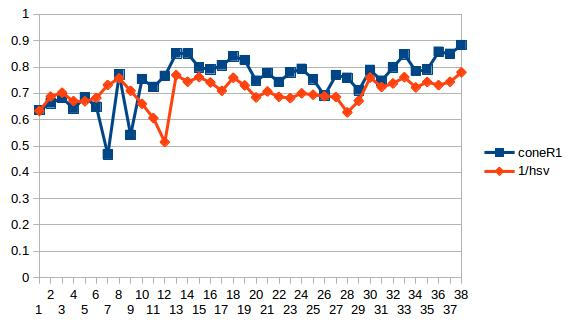
\includegraphics[width=1\linewidth]{figures/correlations/db/campus_hsv.jpg}
%  \caption{aton\_campus ($\alpha_{dB}$)}
%5\end{subfigure}
%\begin{subfigure}{.49\linewidth}
%  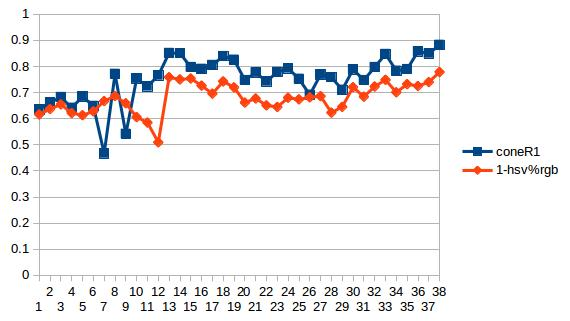
\includegraphics[width=1\linewidth]{figures/correlations/rgb/campus_hsv.jpg}
%  \caption{aton\_campus ($\alpha_{\%\Delta}$)}
%\end{subfigure}
%\hfill
%\begin{subfigure}{.49\linewidth}
%  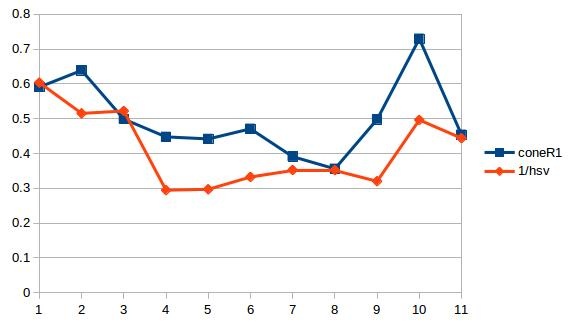
\includegraphics[width=1\linewidth]{figures/correlations/db/pets2_hsv.jpg}
%  \caption{PETS2 ($\alpha_{dB}$)}
%\end{subfigure}
%\begin{subfigure}{.49\linewidth}
%  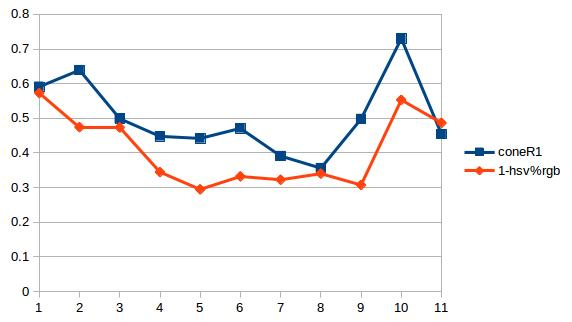
\includegraphics[width=1\linewidth]{figures/correlations/rgb/pets2_hsv.jpg}
%  \caption{PETS2 ($\alpha_{\%\Delta}$)}
%\end{subfigure}

%\caption{Qualitative comparison of $\alpha_{dB}$ (left) and $\alpha_{\%\Delta}$ (right) across datasets. (Full results for each dataset is found in the appendix)}
%\label{fig:corr_compare}
%\end{figure}

The results in Tables \ref{table:corr_db} and \ref{table:corr_rgb} indicate that some datasets benefit \hl{more} from the $\alpha_{dB}$ model, while others \hl{have greater} benefit from the $\alpha_{\%\Delta}$ model. While the correlation found using the two models are comparable, we use the $\alpha_{\%\Delta}$ model in Eqn. \ref{eqn:modelshift}, when calculating the parameter \textit{coneR1}$'$. This is because the $\alpha_{\%\Delta}$ model provides a closer fit to \textit{coneR1}*, in terms of the magnitude shift required \hl{, which is }covered in detail in section \ref{section:model}. An example of this closer fit is found in the qualitative comparison Figure \ref{fig:corr_compare}(a).

\subsection{Correlation Improvements}

In sections \ref{section:brightnessmodels} and \ref{section:lowcSIFT}, we \hl{discuss} \hl{two} indirect environmental properties that may be used to improve correlation\hl{: low-contrast SIFT keypoints and brightness calculation methods.} We conduct sensitivity analysis on the two properties.

Low-contrast SIFT keypoints are analyzed within a frame and are used to produce a scaling factor that is applied to observed attenuation $\alpha_{\%\Delta}$. From this analysis we determine that the low-contrast scaling factor provides boosts to correlation in select datasets, while proving detrimental to others.

We \hl{also} demonstrate that correlation (both $\rho_{dB}$ and $\rho_{\%\Delta}$) are sensitive to varying brightness models, by contrasting their effects across datasets. We show quantifiable and predictable effects on the $\alpha_{dB}$ attenuation model, \hl{that indicate} the HSP and Luma brightness models \hl{are most appropriate for outdoor datsets,} while indoor datasets are not sensitive to varying brightness models. Similar analysis is performed regarding $\rho_{\%\Delta}$; however, \hl{the same trends (outdoor/indoor) are not observed, due to} differences intrinsic to attenuation calculation.

\subsubsection{Low-contrast SIFT Keypoints} \label{section:lowcsensitivity}

Using Eqn. \ref{eqn:ratioratio} defined in section \ref{section:lowcSIFT}, $SIFT_{fg/bg}$ is calculated per frame and multiplied against the observed average attenuation. $SIFT_{\%C}(f)$ represents the ratio of total low contrast SIFT features to normal SIFT features within a frame $f$.

\begin{equation}
SIFT_{fg/bg} = \dfrac{SIFT_{\%C}(fg)}{SIFT_{\%C}(bg)}
\end{equation}

 \hl{The result of the multiplication is stored in the variable $\alpha_{SIFT}$.} Figure \ref{fig:highway1_sift} shows the multiplication's effect on the aton\_highway1 dataset. Figure \ref{fig:corr_diff_sift} and Table \ref{table:corr_diff_sift} detail the effects on correlation ($\rho_{\%\Delta}$) for each dataset.

\begin{figure}
  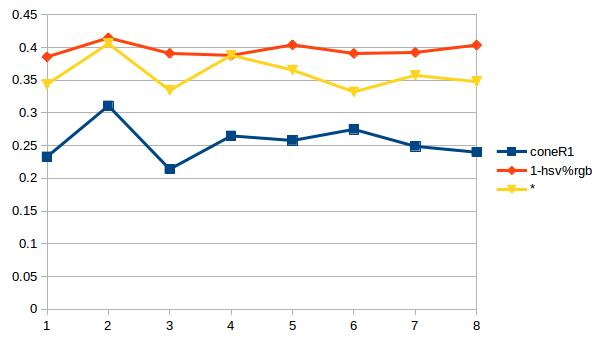
\includegraphics[width=1\linewidth]{figures/highway1_sift.jpg}
\caption{$SIFT_{fg/bg}$ multiplication's effect on correlation for the dataset aton\_highway1. The observed attenuation $\alpha_{\%\Delta}$ (orange), is multiplied by the calculated $SIFT_{fg/bg}$ on a per frame basis. The resultant, shown in yellow, represents a closer fit to \textit{coneR1}* (blue).}
\label{fig:highway1_sift}
\end{figure}

\begin{figure}
  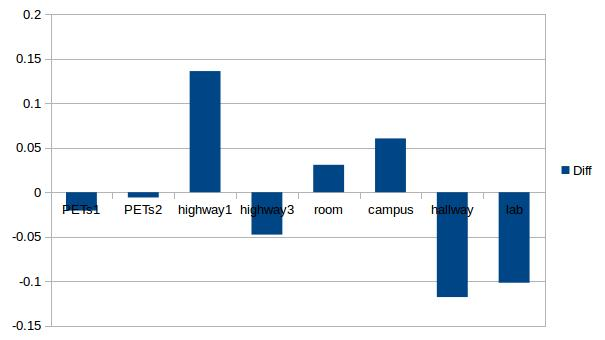
\includegraphics[width=1\linewidth]{figures/sift_correlation_diff.jpg}
\caption{Visualization of correlation shifts ($\rho_{\%\Delta}$) found in Table \ref{table:corr_diff_sift}.}
\label{fig:corr_diff_sift}
\end{figure}

% Table Form (SIFT Diff)
\begin{table}
\centering
\begin{tabular}{ |c|c| }
	\hline
	\textbf{Dataset} & $\rho_{\%\Delta}$ Shift (\%)\\
	\hline
	\hline
	\textbf{PETS1} &  -2.06 \\
	\hline
	\textbf{PETS2} & -0.58 \\
	\hline
	\textbf{aton\_highway1} &  +13.62 \\
	\hline
	\textbf{aton\_highway3} & -4.76  \\
	\hline
	\textbf{aton\_room} & +3.087 \\
	\hline
	\textbf{aton\_campus} & +6.06 \\
	\hline
	\textbf{aton\_hallway} & -11.78 \\
	\hline
	\textbf{aton\_lab} & -10.17 \\
	\hline
\end{tabular}
\caption{Correlation shifts ($\rho_{\%\Delta}$) when $SIFT_{fg/bg}$ is multiplied against observed attenuation $\alpha_{\%\Delta}$.}
\label{table:corr_diff_sift}
\end{table}

Table \ref{table:corr_diff_sift} shows that modulating $\alpha_{\%\Delta}$ by $SIFT_{fg/bg}$ produces inconsistent results. For aton\_highway1, aton\_room, and aton\_campus, the operation produced favorable results. However, for all other datasets it produced unfavorable or negligible results. The datasets that had the greatest improvements, aton\_highway1 and aton\_campus, contain the darkest shadows. Similarly, the most negatively affected datasets, aton\_hallway and aton\_lab, have the faintest shadows. From this observation, we posit that there is a range of shadow brightness in which the saturation channel is affected enough (detailed in section \ref{section:lowcSIFT}) to be detectable as a low-contrast SIFT keypoint, and therefore that range benefits from analyzing low-contrast SIFT keypoints. This validates the assumption that low-contrast SIFT features, while not in direct correlation with \textit{coneR1}*, can provide indirect benefits by improving the existing correlation ($\rho_{\%\Delta}$)\hl{,} depending on the environment. Future work using low-contrast SIFT keypoints begins with determining this threshold.

%%%
%\section{Brightness Models and Correlation} \label{section:brightness_models}
%%%

%\subsection{$\rho_{dB}$ Attenuation Model}
\subsubsection{Brightness Models - $\rho_{dB}$ Attenuation Model}

In addition to differing responses to attenuation models, datasets also respond uniquely to varying brightness models. Figure \ref{fig:brightness_example} illustrates how differing brightness models affect the correlation coefficient of attenuation. Table \ref{table:brightness_corr_db} enumerates the correlative changes experienced by each dataset when subjected to a range of brightness models. These results are illustrated in Figure \ref{fig:brightness_corr_db}.

% example 
\begin{figure}
\centering
\begin{subfigure}{.49\linewidth}
  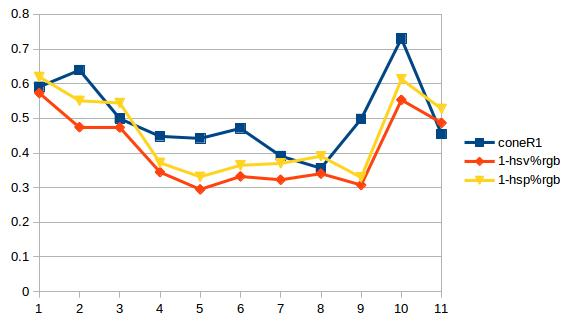
\includegraphics[width=1\linewidth]{figures/brightness/rgb/pets2_hsv_hsp.jpg}
  \caption{PETS2}
\end{subfigure}
\hfill
\begin{subfigure}{.49\linewidth}
  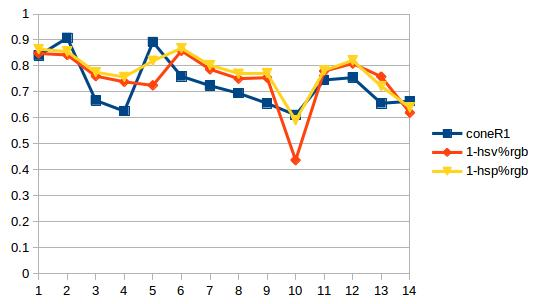
\includegraphics[width=1\linewidth]{figures/brightness/rgb/lab_hsv_hsp.jpg}
  \caption{aton\_lab}
\end{subfigure}

\caption{Example contrasting correlation improvements of the HSP model (yellow) against HSV (red) and \textit{coneR1}* (blue). }
\label{fig:brightness_example}
\end{figure}

% Table Form ((dB) Corr v. Brightness
\begin{table}
\centering
\begin{tabular}{ |c|c|c|c|c|c|c|c| }
	\hline
	\textbf{Dataset} & \textbf{HSV} & \textbf{HSP} & \textbf{HSI} & \textbf{HSL}& \textbf{Y'} & \textbf{Norm} \\
		\textbf{} & $\rho_{dB}$ & $\rho_{dB}$ & $\rho_{dB}$ & $\rho_{dB}$ & $\rho_{dB}$ & $\rho_{dB}$ \\
	\hline
	\hline
	\textbf{PETS1} & 0.199 & 0.227 & 0.202 & 0.190 & 0.222 & 0.205 \\
	\hline
	\textbf{PETS2} & 0.671 & 0.710 & 0.690 & 0.653 & 0.696 & 0.695 \\
	\hline
	\textbf{aton\_highway1} & 0.684 & 0.477 & 0.524 & 0.560 & 0.471 & 0.669 \\
	\hline
	\textbf{aton\_highway3} & 0.742 & 0.814 & 0.795 & 0.780 & 0.816 & 0.773 \\
	\hline
	\textbf{aton\_campus} & 0.359 & 0.483 & 0.430 & 0.416 & 0.487 & 0.420 \\
	\hline
	\hline
	\textbf{aton\_room} & 0.548 & 0.528 & 0.532 & 0.536 & 0.527 & 0.532 \\
	\hline
	\textbf{aton\_hallway} & 0.656 & 0.625 & 0.617 & 0.622 & 0.618 & 0.601 \\
	\hline
	\textbf{aton\_lab} & 0.695 & 0.710 & 0.705 & 0.717 & 0.710 & 0.708 \\
	\hline
\end{tabular}
\caption{Datasets and their correlations to \textit{coneR1}* ($\alpha_{dB}$) against Brightness models. Outdoor (top) and Indoor (bottom) scenes are grouped appropriately.}
\label{table:brightness_corr_db}
\end{table}

% Brightness Models (dB)
\begin{sidewaysfigure}
  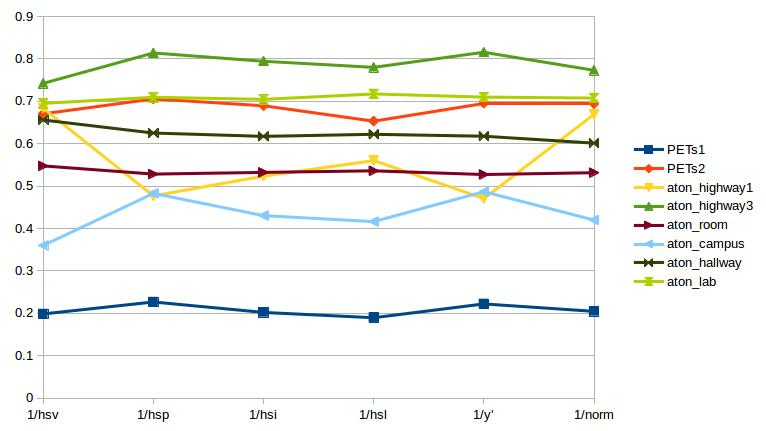
\includegraphics[width=\linewidth]{figures/brightness/db/correlation_x.jpg}
  \caption{Datasets and their correlations (y-axis)to \textit{coneR1}* ($\alpha_{dB}$) against Brightness models (x-axis).}
\label{fig:brightness_corr_db}
\end{sidewaysfigure}

Two distinct response trends are observed in Figure \ref{fig:brightness_corr_db}. These trends are shown in Figure \ref{fig:brightness_indoor_outdoor_db}: outdoor datasets (PETS1, PETS2, aton\_highway3, and aton\_campus) share a similar response to the various brightness models, while indoor datasets (aton\_room, aton\_hallway, and aton\_lab) also share a similar response. Table \ref{table:brightness_corr_db} indicates that $\rho_{dB}$ is sensitive to change in brightness models among outdoor datasets (Figure \ref{fig:brightness_indoor_outdoor_db}(a)), with HSP and Luma (Y') consistently providing the highest correlations. Indoor datasets (Figure \ref{fig:brightness_indoor_outdoor_db}(b)) exhibit negligible sensitivity to brightness model change for $\rho_{dB}$ attenuation. From this indication, we deduce that utilizing either the HSP or Luma brightness model improves correlation ($\rho_{dB}$) for outdoor scenes.

% Brightness Models indoor/outdoor (dB)
\begin{figure}
\centering
\begin{subfigure}{.8\linewidth}
  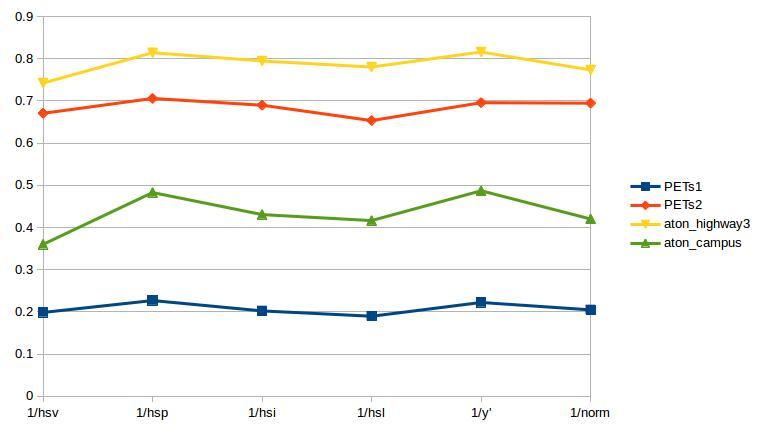
\includegraphics[width=1\linewidth]{figures/brightness/db/correlation_outside.jpg}
  \caption{}
\end{subfigure}
\hfill
\begin{subfigure}{.8\linewidth}
  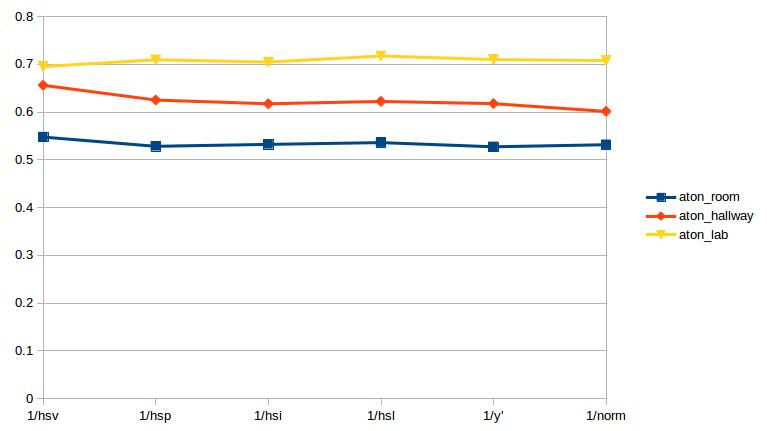
\includegraphics[width=1\linewidth]{figures/brightness/db/correlation_inside.jpg}
  \caption{}
\end{subfigure}

\caption{Outdoor datasets (a) share a common response to varying brightness models. In contrast, indoor datasets (b) share a insensitivity to varying brightness models}.
\label{fig:brightness_indoor_outdoor_db}
\end{figure}

Furthermore, we can predict when to utilize the HSP/Luma models for better (dB) correlation, by measuring the \textit{red-green color bias (defined below) corresponding to shadow regions in a dataset.} The difference in brightness models can be primarily characterized by their individual treatments of color content in a pixel, i.e., both Y' and HSP weight the channels of an RGB image by scaling factors relevant to human perception, while HSV simply takes the largest color channel value as the brightness. We differentiate between the datasets by measuring the average red-green color bias ($\beta^{RG}_{p}$, for pixel $p$) present in shadow pixels. To determine color bias, we use the color shift ($\Delta$RGB) from a foreground shadow pixel to an illuminated background pixel. We define the red-green color bias as the observed blue color shift of a foreground shadow pixel $p$ subtracted from the mean of observed red and green color shifts (Eqn. \ref{eqn:rgb_shift}).

\begin{equation}
\beta^{RG}_{p} = \dfrac{\Delta R_{p} + \Delta G_{p}}{2} - \Delta B_{p}
\label{eqn:rgb_shift}
\end{equation}

This operation is performed on each foreground pixel that is darker than its corresponding background pixel, and averaged into $\beta^{f}_{RG}$, the average red-green color bias per frame. The values of $\beta^{RG}$ are contingent on the representation of the RGB channels in an image. In our study, each channel has a range of $(0, 255)$. As seen in Table \ref{table:rg_bias}, outdoor datasets display consistently higher $\beta^{RG}$ values.

% Table Form RG Color Bias
\begin{table}
\centering
\begin{tabular}{ |c|c| }
	\hline
	\textbf{Dataset} & \textbf{$\beta^{RG}$} \\
	\hline
	\hline
	\textbf{PETS1} & 15.03 \\
	\hline
	\textbf{PETS2} & 7.57 \\
	\hline
	\textbf{aton\_highway1} & 6.69 \\
	\hline
	\textbf{aton\_highway3} & 2.56 \\
	\hline
	\textbf{aton\_campus} & 3.32 \\
	\hline
	\hline
	\textbf{aton\_room} & 1.64 \\
	\hline
	\textbf{aton\_hallway} & -0.26 \\
	\hline
	\textbf{aton\_lab} & 0.35 \\
	\hline
\end{tabular}
\caption{Red-green bias for each dataset. $\beta^{RG}$ represents the average of the $\beta^{RG}_{f}$ for each frame in a dataset. Outdoor (top) and Indoor (bottom) scenes are grouped \hl{together}.}
\label{table:rg_bias}
\end{table}

The exception to this grouping of outdoor and indoor datasets is aton\_highway1, an outdoor dastaset that has a response reciprocal to that of most outdoor environments. Figure \ref{fig:highway1_reciprocal} illustrates the mirrored nature of aton\_highway1's response. 
%In section \ref{section:spectralprop}, we can see aton\_highway1's RGB shift in shadowed regions (Figure \ref{fig:rgshift_outdoor}(c)). 
%The RGB shift is characteristic of an outdoor scene; red, green, and blue channels attenuate by different amounts. However, 
aton\_highway1 contains the darkest cast shadows in relation to its background model. The relative low points, HSP and Luma, both attempt to weight brightness according to color information. The applied weights are the only differing factor in the HSP and Norm methods. Therefore, we conclude that the consideration of color shift is a detriment to aton\_highway1's $\rho_{dB}$ correlations.
%The highest of aton\_highway1's responses, HSV and Norm, both result in an \hl{exaggerated} brightness value in accordance to observed color shifts. HSV is overvalued due to its reliance on one channel. While HSV and Norm serve as relative low points in other outdoor datasets for that reason, the larger calculated brightness attenuation simply provided for a closer relational value with the optimal \textit{coneR1} value in the dark shadowed region.

% aton_highway1 oddity
\begin{figure}
\centering
  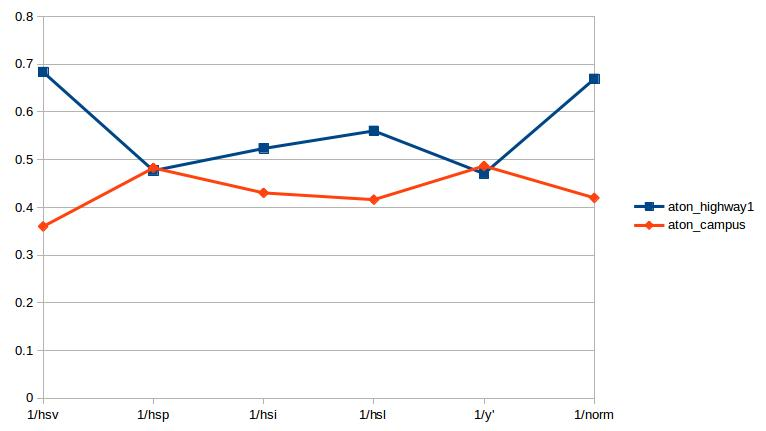
\includegraphics[width=1\linewidth]{figures/brightness/db/highway1_reciprocal.jpg}
\caption{aton\_highway1's response to various brightness models behaves opposite to other outdoor datasets.}
\label{fig:highway1_reciprocal}
\end{figure}

%\subsection{$\rho_{\%\Delta}$ Attenuation Model}
\subsubsection{Brightness Models - $\rho_{\%\Delta}$ Attenuation Model}

Results indicating correlations ($\rho_{\%\Delta}$) per brightness model are enumerated in Table \ref{table:brightness_corr_rgb}. These results are illustrated in Figure \ref{fig:brightness_corr_rgb}.

% Table Form (RGB) Corr v. Brightness
\begin{table}
\centering
\begin{tabular}{ |c|c|c|c|c|c|c|c| }
	\hline
	\textbf{Dataset} & \textbf{HSV} & \textbf{HSP} & \textbf{HSI} & \textbf{HSL}& \textbf{Y'} & \textbf{Norm} \\
	\textbf{} & $\rho_{\%\Delta}$ & $\rho_{\%\Delta}$ & $\rho_{\%\Delta}$ & $\rho_{\%\Delta}$ & $\rho_{\%\Delta}$ & $\rho_{\%\Delta}$ \\
	\hline
	\hline
	\textbf{PETS1} & 0.183 & 0.320 & 0.241 & 0.222 & 0.239 & 0.314 \\
	\hline
	\textbf{PETS2} & 0.743 & 0.741 & 0.746 & 0.717 & 0.747 & 0.732 \\
	\hline
	\textbf{aton\_highway1} & 0.592 & 0.189 & 0.393 & 0.396 & 0.313 & 0.216 \\
	\hline
	\textbf{aton\_highway3} & 0.801 & 0.761 & 0.804 & 0.781 & 0.815 & 0.760 \\
	\hline
	\textbf{aton\_campus} & 0.564 & 0.371 & 0.407 & 0.395 & 0.459 & 0.361 \\
	\hline
	\hline
	\textbf{aton\_room} & 0.622 & 0.618 & 0.621 & 0.621 & 0.623 & 0.616 \\
	\hline
	\textbf{aton\_hallway} & 0.689 & 0.429 & 0.746 & 0.754 & 0.756 & 0.404 \\
	\hline
	\textbf{aton\_lab} & 0.551 & 0.729 & 0.592 & 0.608 & 0.597 & 0.725 \\
	\hline
\end{tabular}
\caption{Datasets and their correlations to \textit{coneR1}* ($\alpha_{\%\Delta}$) against Brightness models. Outdoor (top) and Indoor (bottom) scenes are grouped appropriately.}
\label{table:brightness_corr_rgb}
\end{table}

% Brightness Models (RGB)
\begin{sidewaysfigure}
  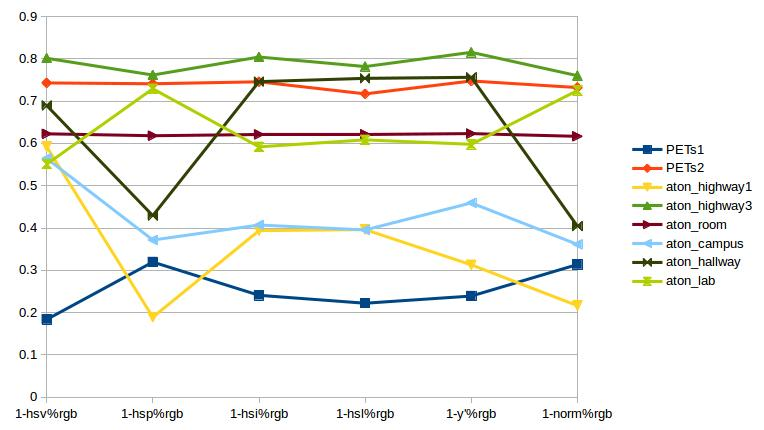
\includegraphics[width=\linewidth]{figures/brightness/rgb/correlation_x.jpg}
  \caption{Datasets and their correlations (y-axis)to \textit{coneR1}* ($\alpha_{\%\Delta}$) against Brightness models (x-axis).}
\label{fig:brightness_corr_rgb}
\end{sidewaysfigure}

% Brightness Models indoor/outdoor (RGB)
\begin{figure}
\centering
\begin{subfigure}{.8\linewidth}
  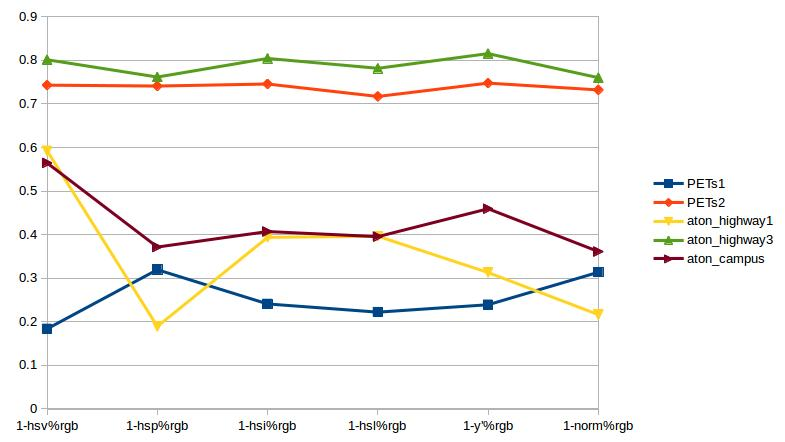
\includegraphics[width=1\linewidth]{figures/brightness/rgb/correlation_outside.jpg}
  \caption{}
\end{subfigure}
\hfill
\begin{subfigure}{.8\linewidth}
  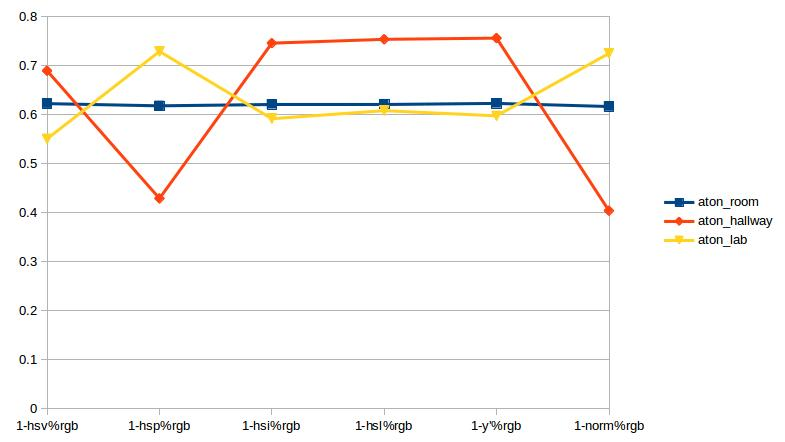
\includegraphics[width=1\linewidth]{figures/brightness/rgb/correlation_inside.jpg}
  \caption{}
\end{subfigure}

\caption{(a) Outdoor datasets. (b) Indoor datasets.}
\label{fig:brightness_indoor_outdoor_rgb}
\end{figure}

It is important to note that Figure \ref{fig:brightness_corr_rgb} does not exhibit the trends indicated by the $\alpha_{dB}$ model in Figure \ref{fig:brightness_corr_db}. The datasets are separated into outdoor/indoor datasets in Figure \ref{fig:brightness_indoor_outdoor_rgb}. Some datasets, such as PETS1, PETS2, aton\_highway3, and aton\_room, demonstrate similar responses to those observed in Figure \ref{fig:brightness_corr_db}. However, aton\_lab, aton\_hallway, and aton\_campus behave erratically in comparison to their corresponding $\alpha_{dB}$ responses. The disparity between the two brightness responses can be attributed to the vectorization of the $\alpha_{\%\Delta}$ model, which calculates the brightness of the vector between a foreground and background pixel. For example, a pixel $p_{1}$ is represented by the RGB values $(25, 50, 75)$, and a second pixel $p_{2}$ is $(75, 50, 25)$. Using the HSV brightness model, we calculate the brightness of each pixel to be 75. The $\alpha_{dB}$ model results in 1.0, or no attenuation. The $\alpha_{\%\Delta}$ model calculates the brightness change of the difference, $p_{2} - p_{1} = (50, 0, -50)$. Using the HSV model, $\alpha_{\%\Delta}$ reports a brightness shift of 50 units, with a resulting attenuation of $50 / 75 = 0.66$. We conclude the attenuation model $\alpha_{\%\Delta}$ is not predictably sensitive to a change in brightness model.

%%%
\section{Parameter Model Results}
%%%

The primary challenge in adapting observed average attenuation into an arbitrary model for shadow removal improvement lies in understanding the necessary translation between observed attenuation and \textit{coneR1}*. Utilizing the formulae specified in section \ref{section:model}, a coarse-grained model is developed. 

Applied to an arbitrary frame, attenuation ($\alpha_{\%\Delta}$) and color magnitude shift ($\Delta$RGB) are analyzed and used to create the necessary translation ($shift_{\alpha}$). This analysis is performed on each brightness model, seen in Figure \ref{fig:model_scatter}. 

% RGB shift per req. shift to optimal
\begin{figure}
\centering
\begin{subfigure}{.49\linewidth}
  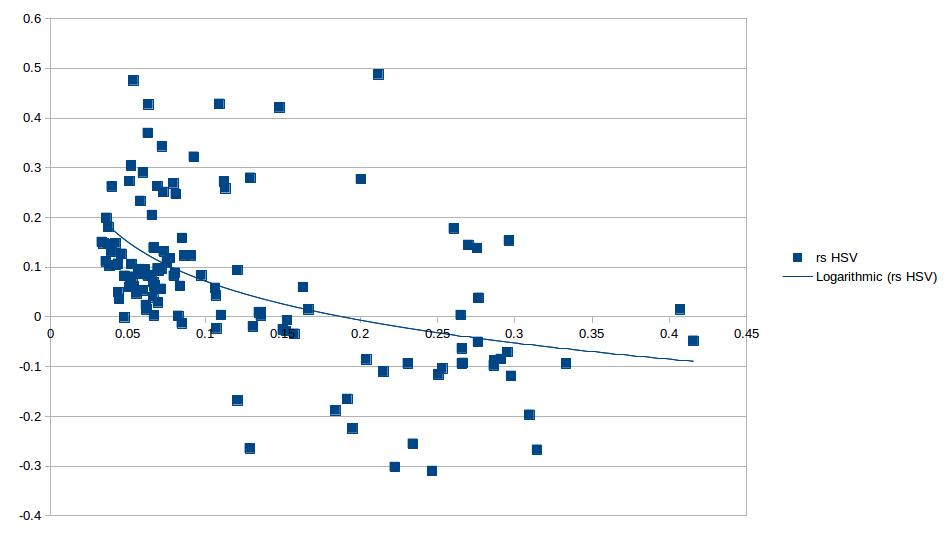
\includegraphics[width=1\linewidth]{figures/model/scatter/model_hsv.jpg}
  \caption{HSV}
\end{subfigure}
\hfill
\begin{subfigure}{.49\linewidth}
  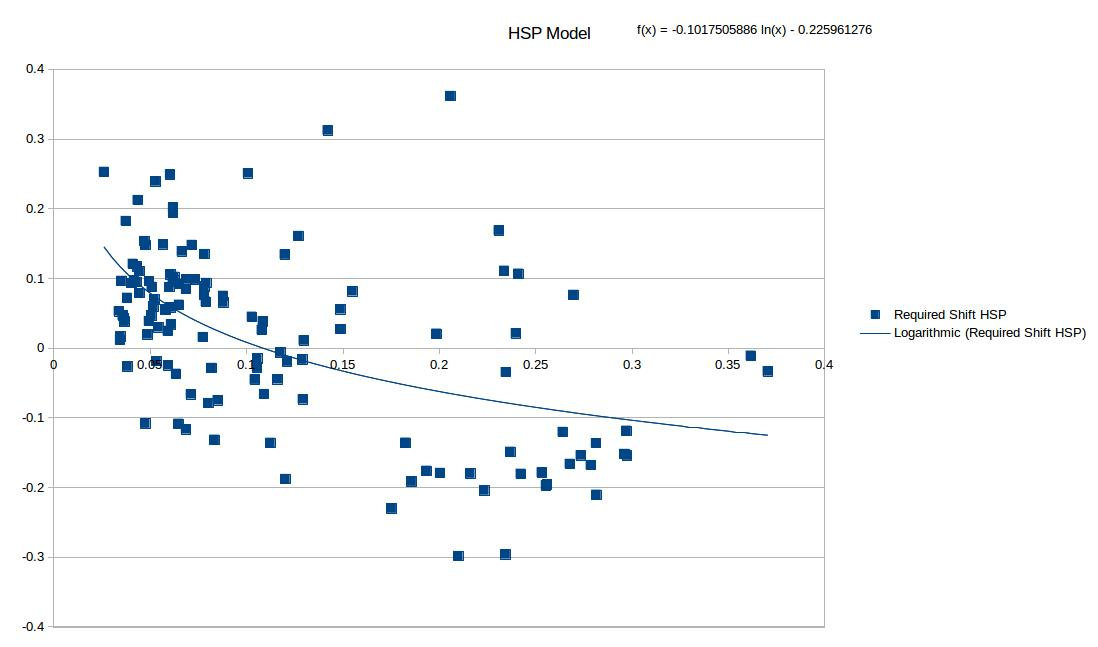
\includegraphics[width=1\linewidth]{figures/model/scatter/model_hsp.jpg}
  \caption{HSP}
\end{subfigure}
\hfill
\begin{subfigure}{.49\linewidth}
  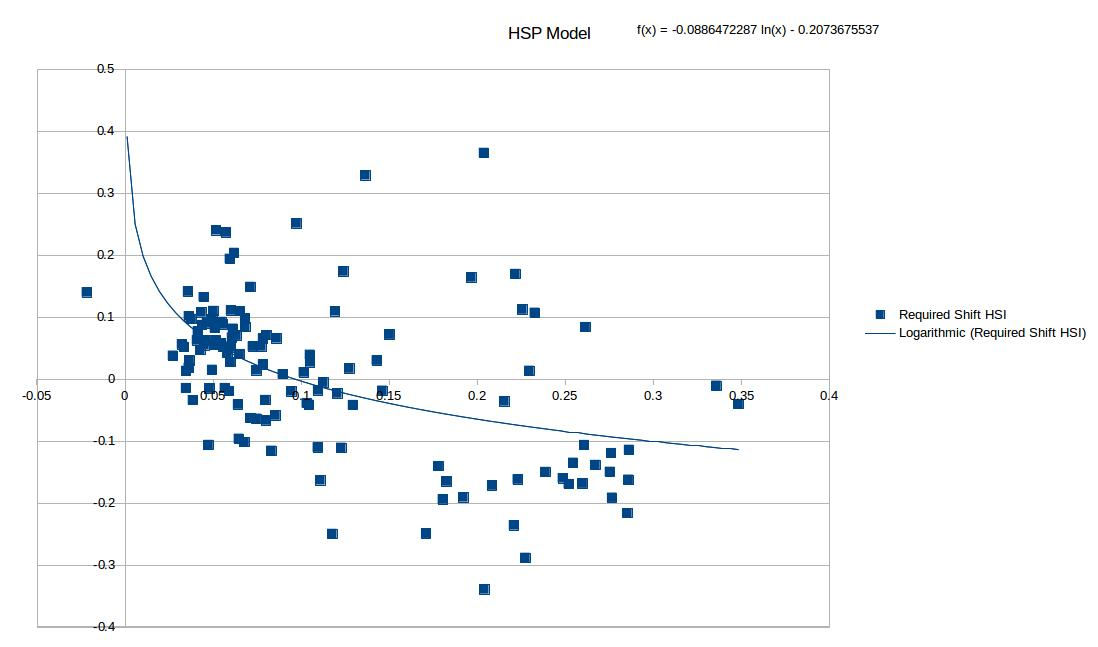
\includegraphics[width=1\linewidth]{figures/model/scatter/model_hsi.jpg}
  \caption{HSI}
\end{subfigure}
\hfill
\begin{subfigure}{.49\linewidth}
  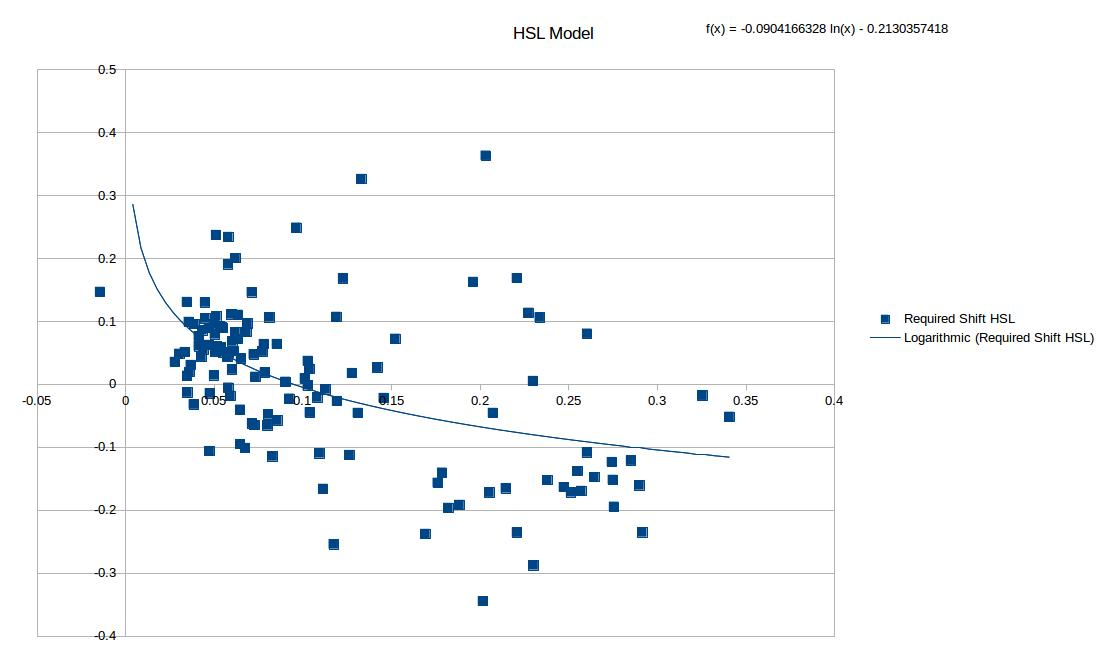
\includegraphics[width=1\linewidth]{figures/model/scatter/model_hsl.jpg}
  \caption{HSL}
\end{subfigure}
\hfill
\begin{subfigure}{.49\linewidth}
  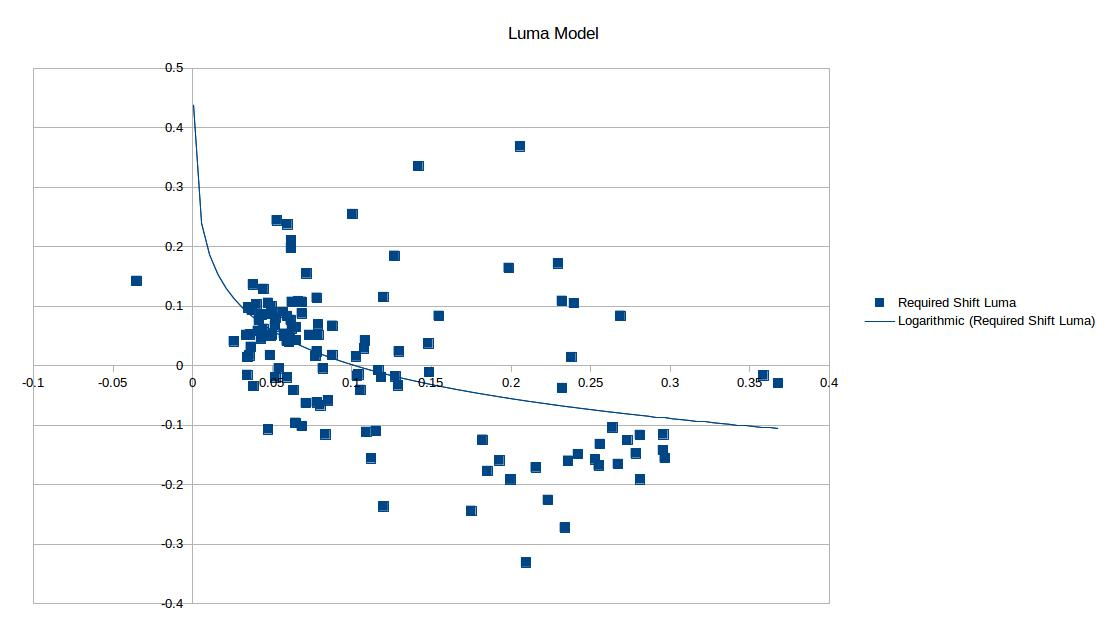
\includegraphics[width=1\linewidth]{figures/model/scatter/model_luma.jpg}
  \caption{Luma (Y')}
\end{subfigure}
\hfill
\begin{subfigure}{.49\linewidth}
  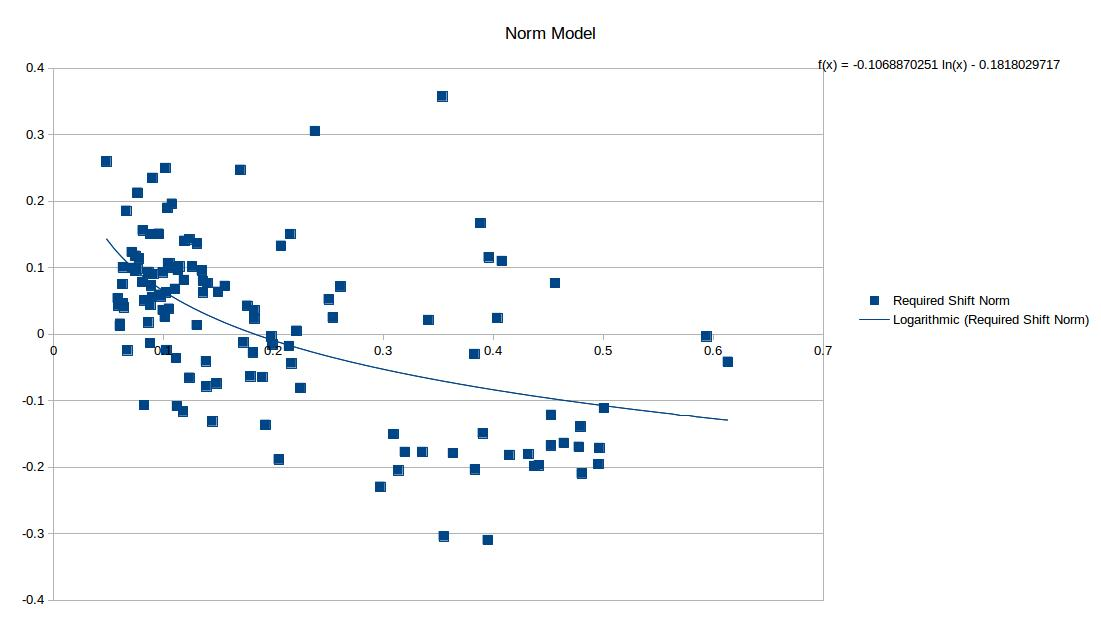
\includegraphics[width=1\linewidth]{figures/model/scatter/model_norm.jpg}
  \caption{Norm}
\end{subfigure}

\caption{For each brightness model, $\Delta$RGB is plotted against $shift_{req.}$. The general model for each brightness calculation is formed through a best-fit logarithm.}
\label{fig:model_scatter}
\end{figure}

Using $\Delta$RGB, $\alpha_{\%\Delta}$, and $shift_{\alpha}$, we calculate the adapted variable \textit{coneR1}$'$. Illustrated results of this model are displayed in Figure \ref{fig:new_coneR1} for the datasets aton\_highway1 and aton\_highway3. The resultant of the model (\textit{coneR1}$'$), shown in orange, retains correlative properties observed prior while providing a reasonable estimate for required translation.

% coneR1 v. newR1
\begin{figure}
  \centering
  \begin{subfigure}{1\linewidth}
  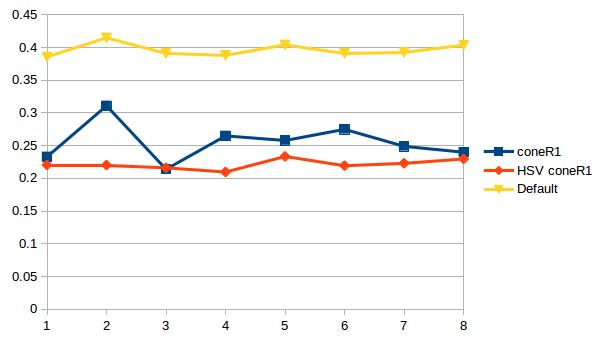
\includegraphics[width=1\linewidth]{figures/model/highway1_calc_coneR1.jpg}
  \caption{aton\_highway1}
\end{subfigure}
\hfill
\begin{subfigure}{1\linewidth}
  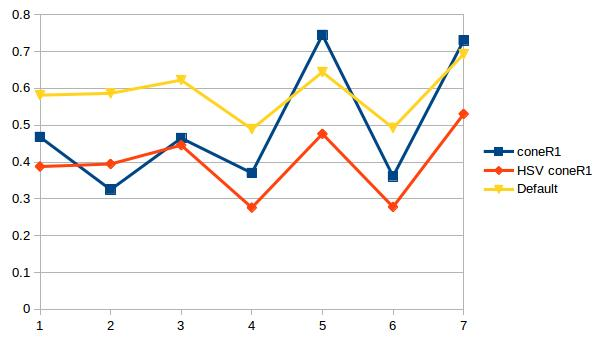
\includegraphics[width=1\linewidth]{figures/model/highway3_calc_coneR1.jpg}
  \caption{aton\_highway3}
\end{subfigure}

\caption{Adaptively tuned \textit{coneR1}$'$ parameter (orange) charted against \textit{coneR1}* (blue) and average attenuation ($\alpha_{\%\Delta}$) (yellow). All results can be found in the appendix.}
\label{fig:new_coneR1}
\end{figure}

\subsection{Analysis}

Figure \ref{fig:bars_hsv_calc} illustrates the resulting detection and discrimination rates of shadow removal using the adapted parameter \textit{coneR1}$'$, contrasting the generated results (orange) with detection/discrimination determined via the original naive method (blue). Detection and discrimination are averaged per frame for each dataset. Quantitative results are shown in Tables \ref{table:quan_results_detect} and \ref{table:quan_results_discrim}.

% detect/discrim calc
\begin{figure}
\centering
\begin{subfigure}{1\linewidth}
  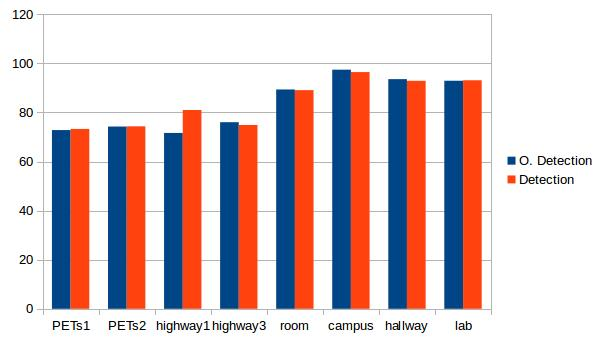
\includegraphics[width=1\linewidth]{figures/model/detect_hsv.jpg}
  \caption{}
\end{subfigure}
\hfill
\begin{subfigure}{1\linewidth}
  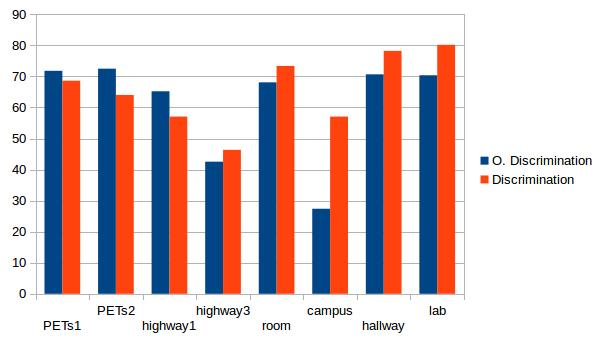
\includegraphics[width=1\linewidth]{figures/model/discrim_hsv.jpg}
  \caption{}
\end{subfigure}

\caption{Average detection (a) and average discrimination (b) calculated using the HSV parameter model, for each dataset.}
\label{fig:bars_hsv_calc}
\end{figure}

% Table Form Quan Results Detect
\begin{table}
\centering
\begin{tabular}{ |c|c|c| }
	\hline
	\textbf{Dataset} & \textbf{$\eta$ (\%)} & \textbf{+/- (\%)} \\
	\hline
	\hline
	\textbf{PETS1} & 73.28 & +0.459 \\
	\hline
	\textbf{PETS2} & 74.34 & +0.056 \\
	\hline
	\textbf{aton\_highway1} & 80.99 & +9.353 \\
	\hline
	\textbf{aton\_highway3} & 74.88 & -1.154 \\
	\hline
	\textbf{aton\_room} & 89.10 & -0.264 \\
	\hline
	\textbf{aton\_campus} & 96.46 & -0.976 \\
	\hline
	\textbf{aton\_hallway} & 92.91 & -0.660 \\
	\hline
	\textbf{aton\_lab} & 93.12 & +0.192 \\
	\hline
\end{tabular}
\caption{Average detection ($\eta$) calculated from the adapted \textit{coneR1}$'$ (left). $\eta$ is compared against original naive detection (\textit{coneR1}$ = 0.3$). The difference (right) is represented as a percentage.}
\label{table:quan_results_detect}
\end{table}

% Table Form Quan Results Discrim
\begin{table}
\centering
\begin{tabular}{ |c|c|c| }
	\hline
	\textbf{Dataset} & \textbf{$\xi$ (\%)} & \textbf{+/- (\%)} \\
	\hline
	\hline
	\textbf{PETS1} & 68.61 & -3.176 \\
	\hline
	\textbf{PETS2} & 64.04 & -8.458 \\
	\hline
	\textbf{aton\_highway1} & 57.05 & -8.172 \\
	\hline
	\textbf{aton\_highway3} & 46.35 & +3.802 \\
	\hline
	\textbf{aton\_room} & 73.36 & +5.278 \\
	\hline
	\textbf{aton\_campus} & 57.05 & +29.67 \\
	\hline
	\textbf{aton\_hallway} & 78.22 & +7.549 \\
	\hline
	\textbf{aton\_lab} & 80.16 & +9.787 \\
	\hline
\end{tabular}
\caption{Average discrimination ($\xi$) calculated from the adapted \textit{coneR1}$'$ (left). $\xi$ is compared against original naive discrimination (\textit{coneR1}$ = 0.3$). The difference (right) is represented as a percentage.}
\label{table:quan_results_discrim}
\end{table}

Results indicate that for a majority of datasets, small amounts of shadow detection accuracy is sacrificed for disproportionate increases in shadow discrimination. Figure \ref{fig:qual_results} qualitatively illustrates shadow removal improvements using the adaptive method for datasets aton\_campus and aton\_room.

\begin{sidewaysfigure}
  \centering
  \begin{subfigure}{.24\linewidth}
  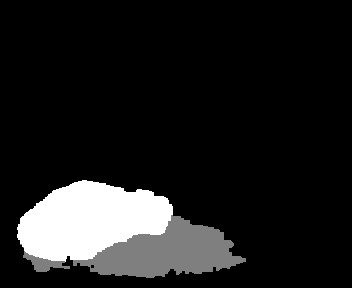
\includegraphics[width=1\linewidth]{figures/model/campus_0061_gt.jpg}
  \caption{Ground Truth}
  \end{subfigure}
  \hfill
  \begin{subfigure}{.24\linewidth}
  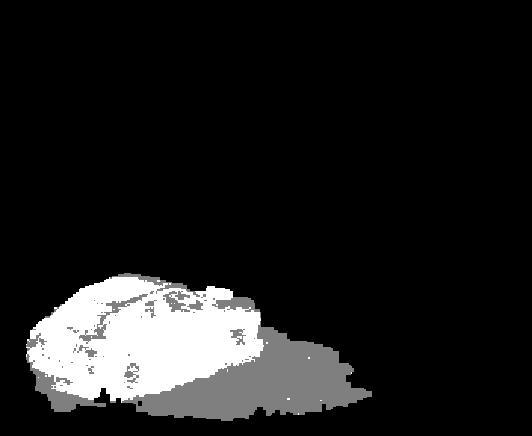
\includegraphics[width=1\linewidth]{figures/model/campus_0061_optimal.jpg}
  \caption{\textit{coneR1}*}
  \end{subfigure}
  \hfill
  \begin{subfigure}{.24\linewidth}
  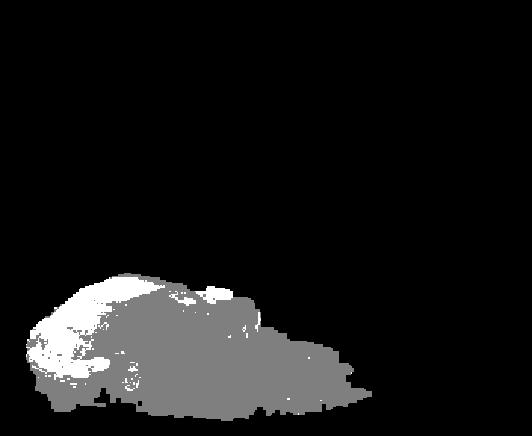
\includegraphics[width=1\linewidth]{figures/model/campus_0061_default.jpg}
  \caption{Default (0.3)}
  \end{subfigure}
  \hfill
  \begin{subfigure}{.24\linewidth}
  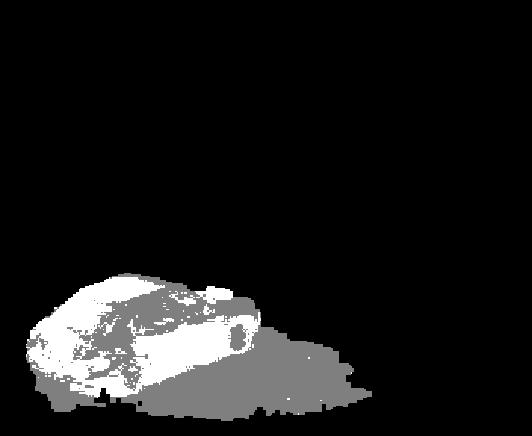
\includegraphics[width=1\linewidth]{figures/model/campus_0061_calc.jpg}
  \caption{\textit{coneR1}$'$}
  \end{subfigure}
  %%%
  \begin{subfigure}{.24\linewidth}
  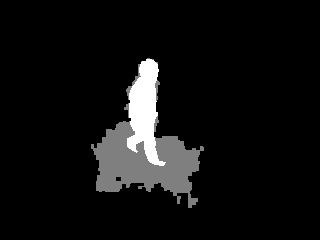
\includegraphics[width=1\linewidth]{figures/model/room_0275_gt.jpg}
  \caption{Ground Truth}
  \end{subfigure}
  \hfill
  \begin{subfigure}{.24\linewidth}
  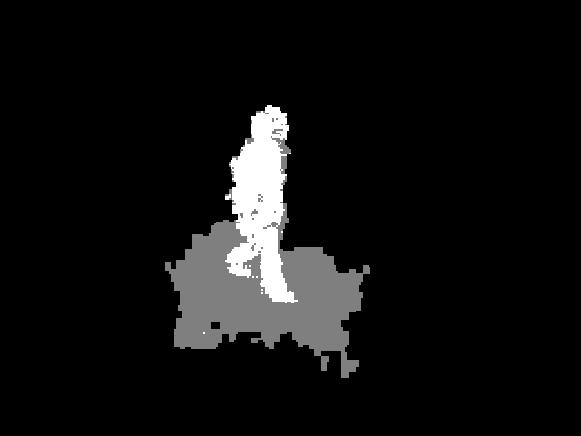
\includegraphics[width=1\linewidth]{figures/model/room_0275_optimal.jpg}
  \caption{\textit{coneR1}*}
  \end{subfigure}
  \hfill
  \begin{subfigure}{.24\linewidth}
  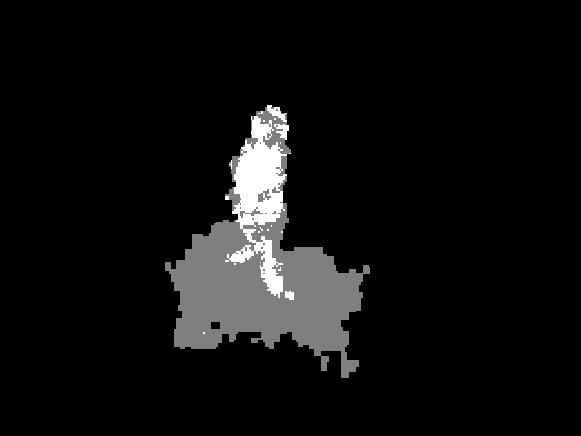
\includegraphics[width=1\linewidth]{figures/model/room_0275_default.jpg}
  \caption{Default (0.3)}
  \end{subfigure}
  \hfill
  \begin{subfigure}{.24\linewidth}
  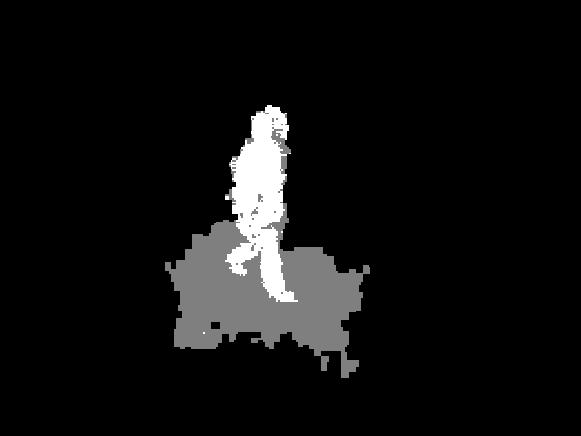
\includegraphics[width=1\linewidth]{figures/model/room_0275_calc.jpg}
  \caption{\textit{coneR1}$'$}
  \end{subfigure}
  
\caption{Qualitative shadow removal improvement. (a - d) feature the aton\_campus dataset, and (e - h) feature the aton\_room datasets.}
\label{fig:qual_results}
\end{sidewaysfigure} 

aton\_highway1 proved anomalous, trading in nearly equal part detection for discrimination, arriving at a net modest positive of 1.2\%. We \hl{hypothesize that is because aton\_highway1 has} the darkest cast shadows. Furthermore, aton\_highway1 attenuates non-linearly (as expected of an outdoor scene), yet \hl{appears} desaturated. The combination of the strong shadows and the low saturation of the frame allows a larger population of candidate shadows pixels to be gathered. Due to these conditions, foreground \textit{object} pixels are more likely to appear identical to shadow pixels, in both color information and relative distance from its background pixel. The confluence of these scene characteristics renders aton\_highway1 less predictable than other datasets.

PETS1 and PETS2 also do not conform to the upward trends seen in the majority of datasets. In the case of PETS1, the low correlation coefficient infers the poor detection/discrimination observed. More interestingly, PETS2 experiences the same degradation of performance as PETS1, but has a much stronger correlation coefficient, seen in Table \ref{table:corr_rgb}. This decoupling of correlation and accuracy stems from \hl{the necessary translation of the observed average attenuation by the generalized adaptation model}. This is illustrated in Figure \ref{fig:pets2_translate}. The model overcompensates for observed color shift ($\Delta$RGB) in PETS2, \hl{because of} the illumination change in the dataset. The misrepresentation of attenuation (and thereby $\Delta$RGB) of cast shadows in PETS2 results in the unnecessary 'downward' translation, impacting PETS2's shadow discrimination accuracy. \hl{This may be solved using techniques for rapid illumination change compensation [\ref{Bales}], explained in section \ref{section:futurework}}.

\begin{figure}
  \centering
  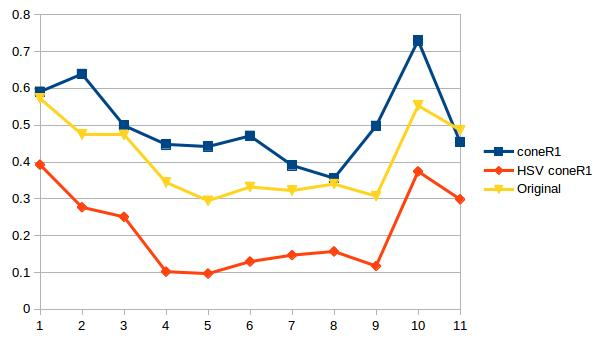
\includegraphics[width=1\linewidth]{figures/model/pets2_translate.jpg}
\caption{For PETS2, the adapted parameter \textit{coneR1}$'$ (orange) is erroneously shifted downwards. The originally observed attenuation ($\alpha_{\%\Delta}$) is shown in yellow.}
\label{fig:pets2_translate}
\end{figure} 

%\subsection{Brightness Models and Shadow Removal}

%It is noted in section \ref{section:brightness_models} that the correlative changes observed in varying brightness models are not consistent from the \hl{$\alpha_{dB}$} to the \hl{$\alpha_{\%\Delta}$} model of attenuation. While correlation coefficient and shadow removal improvement are often related, it is entirely possible to observe cases in which the opposite is true. For example, two vectors are perfectly correlated, $a^T$ = [20, 10] and $b^T$ = [10, 0]. By increasing $b^T$ to [10, 10], the vectors' correlation coefficient is greatly reduced, while their overall fit has been improved. The following results demonstrate this concept, uncoupling the correlation changes recorded in section \ref{section:brightness_models} from shadow removal improvement. Figure \ref{fig:pets1_bars_calc_all} illustrates detection (blue) and discrimination (orange) rates within a dataset across varying brightness \hl{model}, \hl{using the $\alpha_{\%\Delta}$ attenuation model}.

% HSV, HSP, etc for one dataset
%\begin{figure}
%\centering
%  \begin{subfigure}{1\linewidth}
%  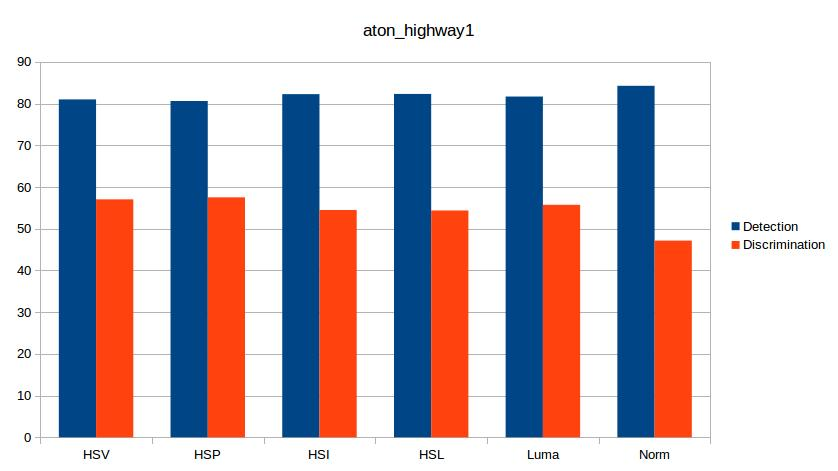
\includegraphics[width=1\linewidth]{figures/model/highway1_all_brightness_models.jpg}
%  \caption{aton\_highway1}
%\end{subfigure}
%\hfill
%  \begin{subfigure}{1\linewidth}
%  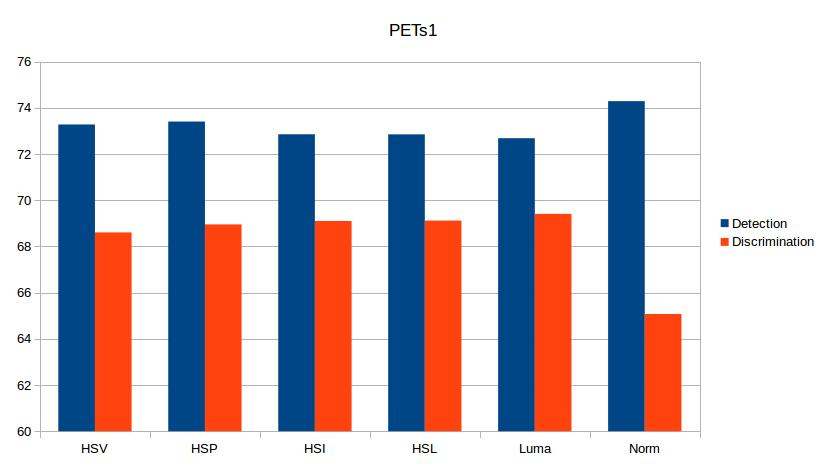
\includegraphics[width=1\linewidth]{figures/model/pets1_all_brightness_models.jpg}
%  \caption{PETS1}
%\end{subfigure}
%\caption{Detection (blue) and Discrimination (orange) for each brightness model. Full results for all datasets can be found in the appendix.}
%\label{fig:pets1_bars_calc_all}
%\end{figure}

%The effect of varying brightness models on shadow removal improvement adheres to \hl{correlation} trends, identified in section \ref{section:brightness_models}, \hl{for the datasets aton\_room, aton\_campus, aton\_hallway, and aton\_lab. For these datasets, shadow detection accuracy is improved up to 2\%, and shadow discrimination is improved up to 3\%. For the remaining datasets, varying the brightness model imparted change on only the correlation, and did not affect detection or discrimination. These results indicate that while correlation ($\rho_{\%\Delta}$) is sensitive to brightness model change, the resulting shadow removal itself is not consistently sensitive to correlation changes. Furthermore, the datasets that are sensitive to change in brightness model are only affected marginally, in contrast to the correlation responses in section \ref{section:brightness_models}.}